\documentclass[10pt,a4paper]{article}
\usepackage[utf8]{inputenc}
\usepackage[T1]{fontenc}
\usepackage[ngerman]{babel}
\usepackage{amsmath}
\usepackage{amsfonts}
\usepackage{amssymb}
\usepackage{graphicx}


\author{Gruppe 02}
\title{Pflichtenheft}
\begin{document}

	\subsection{Adminbereich}
	\subsubsection{Benutzer sperren}
	\begin{figure}[h]
		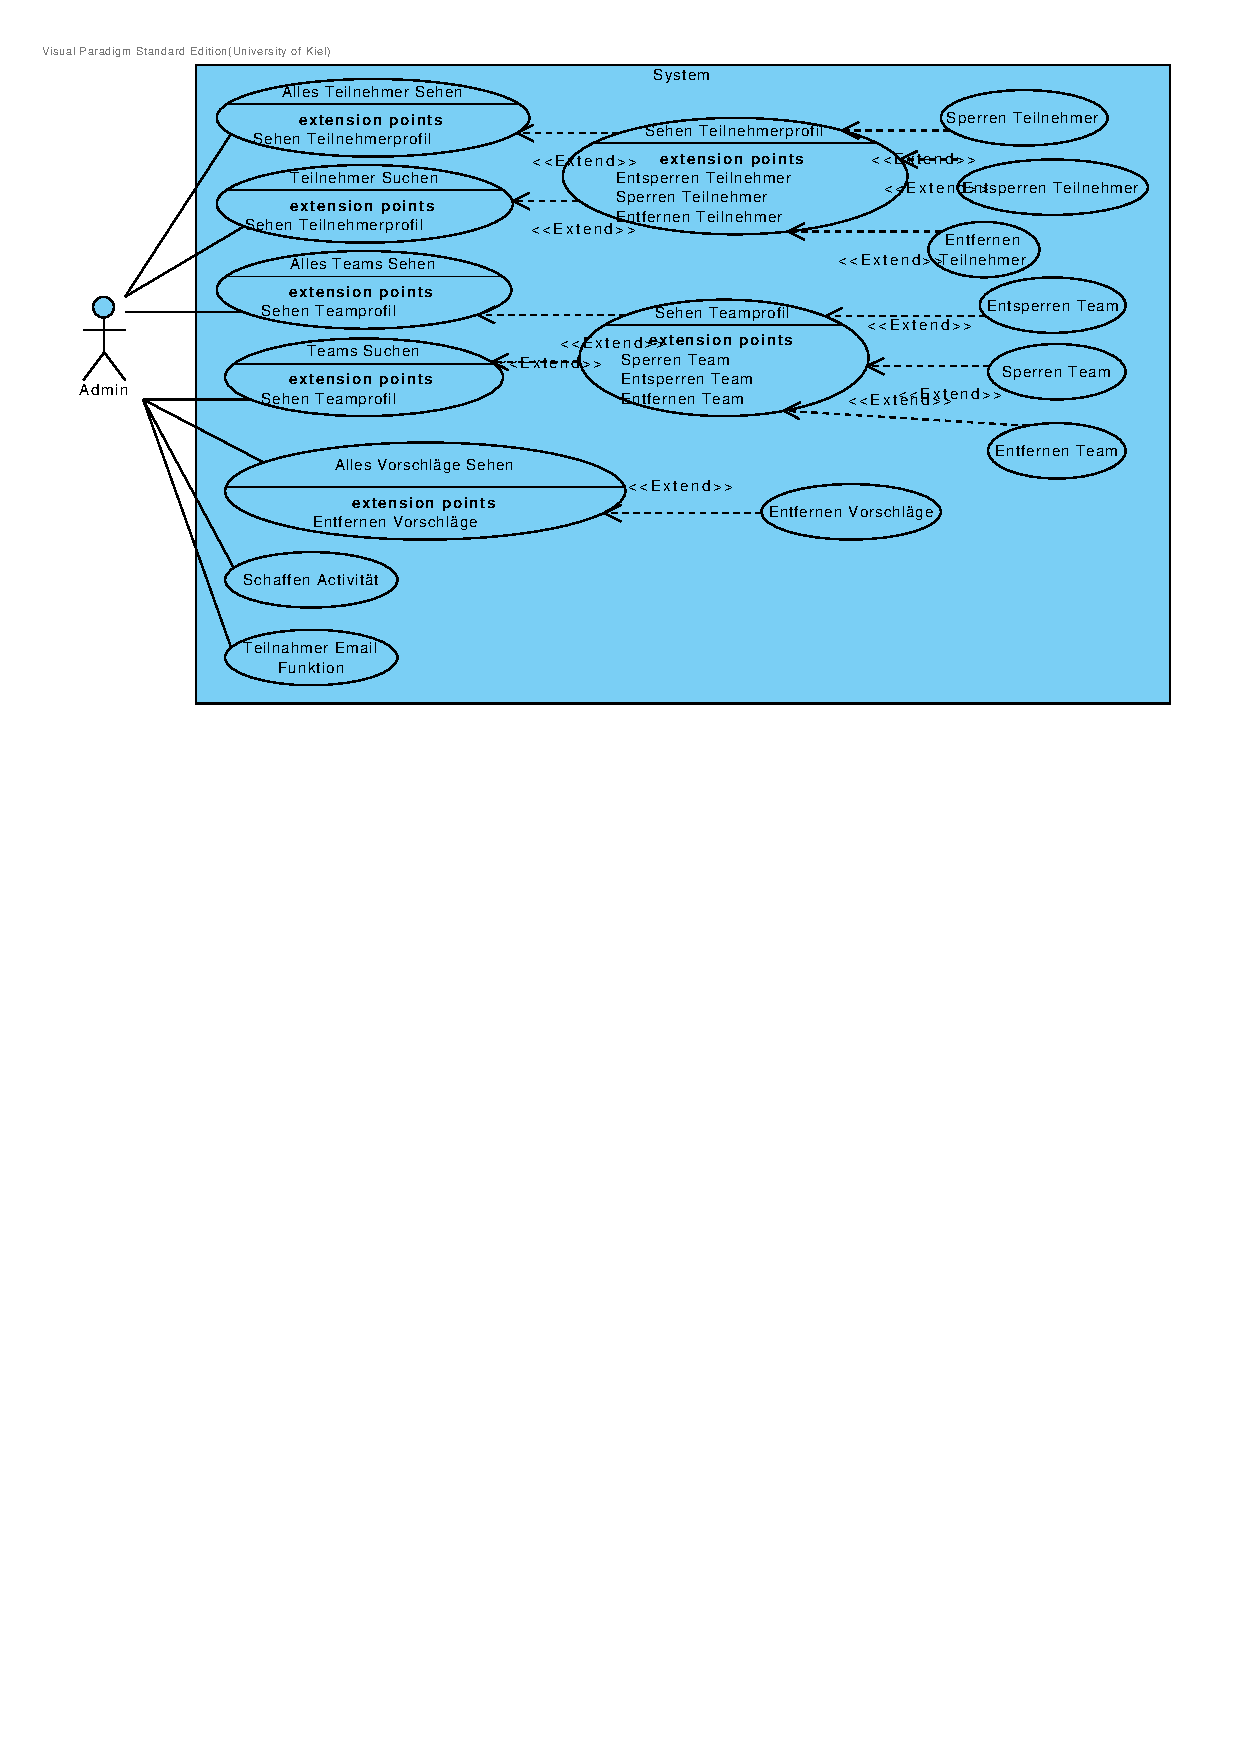
\includegraphics[width=\linewidth]{gfx/webseite/adminbereich.pdf}
	\end{figure}
	\begin{tabular}{|l|p{.5\linewidth}|}
	\hline Use Case Nummer & 1.7.1 \\ 
	\hline Use Case Name & Benutzer sperren \\ 
	\hline Initiierender Akteur & Admin \\
	\hline Weitere Akteure & Benutzer \\
	\hline Kurzbeschreibung & Der Admin wählt einen Benutzer aus und sperrt ihn, sodass dieser nicht mehr auf die Anwendung zugreifen kann \\
	\hline Vorbedingung & Administrator ist als solcher angemeldet \\
	\hline Nachbedingung & Das Profil des ausgewählten Benutzers ist gesperrt \\
	\hline \multicolumn{2}{|c|}{Funktionalität des Use Cases}\\
	\hline Ablauf & \begin{itemize}
			\item Admin sucht den zu sperrenden Benutzer raus\\
			\item Admin wählt Benutzer sperren aus\\
			\item Admin bestätigt die Entscheidung den Benutzer zu sperren\\
		\end{itemize} \\
	\hline Alternativen & - \\
	\hline Ausnahmen & - \\
	\hline Benutzte Use Cases & \begin{itemize}
			\item Benutzerliste einsehen\\
			\item Benutzer suchen\\
			\item Benutzerprofil ansehen\\
		\end{itemize} \\
	\hline \multicolumn{2}{|c|}{Weitere Informationen} \\
	\hline Spezielle Anforderungen &  \\
	\hline Annahmen &  \\
	\hline
	\end{tabular}
	
	\subsubsection{Benutzer reaktivieren}
	\begin{tabular}{|l|p{.5\linewidth}|}
	\hline Use Case Nummer & 1.7.2 \\ 
	\hline Use Case Name & Benutzer reaktivieren \\ 
	\hline Initiierender Akteur & Admin \\
	\hline Weitere Akteure & Benutzer \\
	\hline Kurzbeschreibung & Der Admin wählt einen zur Zeit gesperrten Benutzer aus und reaktiviert ihn, sodass dieser wieder Zugriff auf die Anwendung hat \\
	\hline Vorbedingung & Administrator als solcher angemeldet \\
	\hline Nachbedingung & Der reaktivierte Benutzer hat wieder vollen Zugriff auf die Anwendung und sein Profil ist für andere wieder einsehbar \\
	\hline \multicolumn{2}{|c|}{Funktionalität des Use Cases}\\
	\hline Ablauf & \begin{itemize}
			\item Admin wählt einen gesperrten Benutzer aus\\
			\item Der Admin reaktiviert den entsprechenden Benutzer\\
			\item Der Admin bestätigt, dass er diesen Benutzer wirklich reaktivieren möchte\\
		\end{itemize} \\
	\hline Alternativen & \\
	\hline Ausnahmen &  \\
	\hline Benutzte Use Cases & \begin{itemize}
			\item Benutzerliste einsehen\\
			\item Benutzerprofil ansehen\\
		\end{itemize} \\
	\hline \multicolumn{2}{|c|}{Weitere Informationen} \\
	\hline Spezielle Anforderungen &  \\
	\hline Annahmen &  \\
	\hline
	\end{tabular}
	
	\subsubsection{Benutzer löschen}
	\begin{tabular}{|l|p{.5\linewidth}|}
	\hline Use Case Nummer & 1.7.3 \\ 
	\hline Use Case Name & Benutzer löschen \\ 
	\hline Initiierender Akteur & Admin \\
	\hline Weitere Akteure & User \\
	\hline Kurzbeschreibung & Der Administrator wählt einen Benutzer aus und löscht diesen komplett aus dem System \\
	\hline Vorbedingung & Administrator ist als solcher angemeldet \\
	\hline Nachbedingung & Das Profil des gelöschten Teilnehmers ist aus dem System entfernt \\
	\hline \multicolumn{2}{|c|}{Funktionalität des Use Cases}\\
	\hline Ablauf & \begin{itemize}
			\item Admin wählt den zu löschenden Benutzer aus\\
			\item Der Admin löscht den betreffenden Benutzer\\
			\item Der Admin bestätigt, dass er den Benutzer wirklich löschen möchte\\
		\end{itemize} \\
	\hline Alternativen & Der Admin sucht den zu löschenden Benutzer über die Suchfunktion\\
	\hline Ausnahmen &  \\
	\hline Benutzte Use Cases & \begin{itemize}
			\item Benutzerliste einsehen\\
			\item Benutzer suchen
			\item Benutzerprofil einsehen\\
		\end{itemize} \\
	\hline \multicolumn{2}{|c|}{Weitere Informationen} \\
	\hline Spezielle Anforderungen &  \\
	\hline Annahmen &  \\
	\hline
	\end{tabular} 
	
	\subsubsection{Team löschen}
	\begin{tabular}{|l|p{.5\linewidth}|}
	\hline Use Case Nummer & 1.7.4 \\ 
	\hline Use Case Name & Team löschen \\ 
	\hline Initiierender Akteur & Admin \\
	\hline Weitere Akteure & User \\
	\hline Kurzbeschreibung & Der Administrator hat die Möglichkeit ein Team zu löschen, wobei die einzelnen Mitglieder jedoch nicht automatisch gelöscht werden \\
	\hline Vorbedingung & Als Administrator angemeldet \\
	\hline Nachbedingung & Das Team wurde aus dem System entfernt, die einzelnen Benutzer sind noch vorhanden, jedoch nun ohne Teamzugehörigkeit \\
	\hline \multicolumn{2}{|c|}{Funktionalität des UseCases}\\
	\hline Ablauf & \begin{itemize}
			\item Admin wählt das zu löschende Team aus\\
			\item Der Admin löscht das Team\\
			\item Der Admin bestätigt, dass er das ausgewählte Team wirklich löschen möchte\\
		\end{itemize} \\
	\hline Alternativen & Alternativ kann der Admin das Team über die Suche finden \\
	\hline Ausnahmen &  \\
	\hline Benutzte Use Cases & \begin{itemize}
			\item Teamliste einsehen\\
			\item Team suchen\\
			\item Teamprofil einsehen\\
		\end{itemize} \\
	\hline \multicolumn{2}{|c|}{Weitere Informationen} \\
	\hline Spezielle Anforderungen &  \\
	\hline Annahmen &  \\
	\hline
	\end{tabular}
	
	\subsubsection{Vorschlag in Aktivität umwandeln}
	\begin{tabular}{|l|p{.5\linewidth}|}
	\hline Use Case Nummer & 1.7.5 \\ 
	\hline Use Case Name & Vorschlag in Aktivität umwandeln \\ 
	\hline Initiierender Akteur & Admin \\
	\hline Weitere Akteure & \\
	\hline Kurzbeschreibung & Der Admin kann einen besonders guten Vorschlag in eine Aktivität umwandeln, die dann allen Benutzern zur Verfügung steht \\
	\hline Vorbedingung & Als Administrator angemeldet \\
	\hline Nachbedingung & Der umgewandelte Vorschlag ist nicht mehr bei den Vorschlägen aufgeführt, dafür jedoch in der Aktivitätenliste \\
	\hline \multicolumn{2}{|c|}{Funktionalität des UseCases}\\
	\hline Ablauf & \begin{itemize}
			\item Der Admin wählt den Vorschlag aus, den er zu einer Aktivität abändern möchte
			\item Der Admin trägt die noch benötigten Informationen in die Bearbeitungsmaske ein und speichert die Aktivität
		\end{itemize} \\
	\hline Alternativen &  \\
	\hline Ausnahmen & \begin{itemize}
			\item Der Vorgang kann nicht abgeschlossen werden, wenn nicht alle benötigten Informationsfelder ausgefüllt sind\\
			\item Der Vorgang kann nicht abgeschlossen werden, wenn der eingegebene Titel oder Beschreibungstext zu lang sind\\
			\item Der Vorgang kann nicht abgeschlossen werden, wenn der eingegebene Punktwert kein Integer zwischen 1 und 5 ist\\
		\end{itemize} \\
	\hline Benutzte Use Cases &  \\
	\hline \multicolumn{2}{|c|}{Weitere Informationen} \\
	\hline Spezielle Anforderungen &  \\
	\hline Annahmen & Der Admin achtet darauf, dass die Eingaben korrekt und sinnvoll sind \\
	\hline
	\end{tabular}
	
	\subsubsection{Vorschlag löschen}
	\begin{tabular}{|l|p{.5\linewidth}|}
	\hline Use Case Nummer & 1.7.6 \\ 
	\hline Use Case Name & Vorschlag löschen \\ 
	\hline Initiierender Akteur & Admin \\
	\hline Weitere Akteure & \\
	\hline Kurzbeschreibung & Der Administrator wählt einen unpassenden oder anderweitig überflüssigen Vorschlag aus und löscht diesen \\
	\hline Vorbedingung & Als Administrator angemeldet \\
	\hline Nachbedingung & Der Vorschlag erscheint auf der Vorschlagsseite nicht mehr und ist aus dem System gelöscht \\
	\hline \multicolumn{2}{|c|}{Funktionalität des UseCases}\\
	\hline Ablauf & \begin{itemize}
			\item Admin wählt den zu löschenden Vorschlag aus\\
			\item Der Admin bestätigt, dass er den Vorschlag löschen möchte\\
		\end{itemize} \\
	\hline Alternativen &  \\
	\hline Ausnahmen &  \\
	\hline Benutzte Use Cases & Vorschlagsliste ansehen\\
	\hline \multicolumn{2}{|c|}{Weitere Informationen} \\
	\hline Spezielle Anforderungen &  \\
	\hline Annahmen &  \\
	\hline
	\end{tabular}
	
	\subsubsection{neue Aktivität erzeugen}
	\begin{tabular}{|l|p{.5\linewidth}|}
		\hline Use Case Nummer & 1.7.7 \\ 
		\hline Use Case Name & neue Aktivität erzeugen \\ 
		\hline Initiierender Akteur & Admin \\
		\hline Weitere Akteure & \\
		\hline Kurzbeschreibung & Der Administrator fügt der Liste der verfügbaren Aktivitäten eine neue hinzu (nicht notwendigerweise vorher als Vorschlag vorhanden) \\
		\hline Vorbedingung & Als Administrator angemeldet \\
		\hline Nachbedingung & Die Aktivitätenliste ist um eine Aktivität erweitert \\
		\hline \multicolumn{2}{|c|}{Funktionalität des UseCases}\\
		\hline Ablauf & \begin{itemize}
			\item Admin wählt auf der Aktivitätenseite "neue Aktivität hinzufügen"\\
			\item Der Admin füllt das entsprechende Formular mit den benötigten Informationen aus\\
			\item Der Admin speichert die neue Aktivität\\
		\end{itemize} \\
		\hline Alternativen &  \\
		\hline Ausnahmen & Falsche Eingaben sorgen dafür, dass die Aktivität nicht gespeichert werden kann \\
		\hline Benutzte Use Cases & Aktivitätenliste ansehen\\
		\hline \multicolumn{2}{|c|}{Weitere Informationen} \\
		\hline Spezielle Anforderungen &  \\
		\hline Annahmen & Der Admin füllt das Formular korrekt und sinnvoll aus \\
		\hline
	\end{tabular}
	
	\subsubsection{Alle Benutzer per E-Mail benachrichtigen}
	\begin{tabular}{|l|p{.5\linewidth}|}
		\hline Use Case Nummer & 1.7.8 \\ 
		\hline Use Case Name & Alle Benutzer per E-Mail benachrichtigen \\ 
		\hline Initiierender Akteur & Admin \\
		\hline Weitere Akteure & Benutzer \\
		\hline Kurzbeschreibung & Der Administrator hat die Möglichkeit alle Benutzer per Mail zu kontaktieren (für Hinweise bzgl. Challenges etc.) \\
		\hline Vorbedingung & Als Administrator angemeldet \\
		\hline Nachbedingung & - \\
		\hline \multicolumn{2}{|c|}{Funktionalität des UseCases}\\
		\hline Ablauf & \begin{itemize}
			\item Admin wählt bei seinen Optionen "Nachricht an alle Benutzer"\\
			\item Der Admin füllt das entsprechende Formular mit der Nachricht aus\\
			\item Der Admin verschickt die Nachricht automatisch per Rundmail an alle Teilnehmer\\
		\end{itemize} \\
		\hline Alternativen &  \\
		\hline Ausnahmen & \\
		\hline Benutzte Use Cases & \\
		\hline \multicolumn{2}{|c|}{Weitere Informationen} \\
		\hline Spezielle Anforderungen &  \\
		\hline Annahmen &  \\
		\hline
	\end{tabular}
	
\end{document}